\begin{exercice*}
    \begin{enumerate}
        \item Justifier que les triangles sont isométriques.
        
        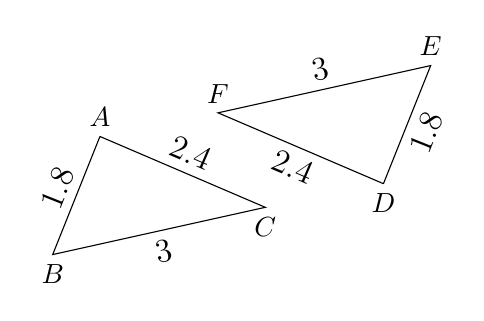
\begin{tikzpicture}[scale = 0.3]
            % \draw[help lines, color=gray!30, dashed] (0,0) grid (18,10);
            \coordinate[label=above:$A$] (A) at (3,6);
            \coordinate[label=below:$B$] (B) at (1,1);
            \coordinate[label=below:$C$] (C) at (10,3);
            \coordinate[label=below:$D$] (D) at (15,4);
            \coordinate[label=above:$E$] (E) at (17,9);
            \coordinate[label=above:$F$] (F) at (8,7);
            \draw (A) -- node[sloped,above] {\large\Lg{1.8}} (B) -- node[sloped,below] {\large\Lg{3}} (C) -- node[sloped,above] {\large\Lg{2.4}} (A);
            \draw (D) -- node[sloped,below] {\large\Lg{1.8}} (E) -- node[sloped,above] {\large\Lg{3}} (F) -- node[sloped,below] {\large\Lg{2.4}} (D);
        \end{tikzpicture}
        \item Justifier que les triangles ne sont pas isométriques.
        
        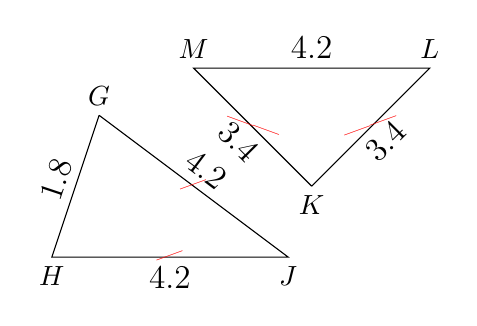
\begin{tikzpicture}[scale = 0.3]
            % \draw[help lines, color=gray!30, dashed] (0,0) grid (18,10);
            \coordinate[label=above:$G$] (A) at (3,7);
            \coordinate[label=below:$H$] (B) at (1,1);
            \coordinate[label=below:$J$] (C) at (11,1);
            \coordinate[label=below:$K$] (D) at (12,4);
            \coordinate[label=above:$L$] (E) at (17,9);
            \coordinate[label=above:$M$] (F) at (7,9);
            \draw (A) -- node[sloped,above] {\large\Lg{1.8}} (B) -- node[sloped,below] {\large\Lg{4.2}} (C) -- node[sloped,above] {\large\Lg{4.2}} (A);
            \draw (D) -- node[sloped,below] {\large\Lg{3.4}} (E) -- node[sloped,above] {\large\Lg{4.2}} (F) -- node[sloped,below] {\large\Lg{3.4}} (D);
            \draw [color=red] (6,1) node[anchor = center, rotate = 20] {|};% (B)(C)
            \draw [color=red] (7,4) node[anchor = center, rotate = 20] {|};% (A)(C)
            \draw [color=red] (9.5,6.5) node[anchor = center, rotate = -20] {||};% (M)(K)
            \draw [color=red] (14.5,6.5) node[anchor = center, rotate = 20] {||};% (L)(K)
        \end{tikzpicture}
    \end{enumerate}
\end{exercice*}
\begin{corrige}
    %\setcounter{partie}{0} % Pour s'assurer que le compteur de \partie est à zéro dans les corrigés
    \phantom{rrr}    
    \begin{multicols}2
        \begin{enumerate}
            \item $AB=DE$; $AC=FD$ et $BC=EF$, les côtés des triangles $ABC$ et $DEF$ sont deux à deux égaux
            
            donc \psshadowbox{ils sont isométriques.}
            \item $GH=GJ$, les longueurs des côtés du triangle $GHJ$ sont donc \Lg{3.2}; \Lg{3.2} et \Lg{2.7}.
            
            $KM=KL$ , les longueurs des côtés du triangle $MLK$ sont donc \Lg{3.2}; \Lg{2.7} et \Lg{2.7}.

            Les côtés des triangles $GHJ$ et $MLK$ ne sont pas deux à deux égaux
            
            donc \psshadowbox{ils ne sont pas isométriques.}
        \end{enumerate}
    \end{multicols}
\end{corrige}

